\documentclass{article}
\usepackage{graphicx} % Required for inserting images
\usepackage{hyperref} % Required for crosslink
\usepackage{subcaption} % Required for subcaption for figures
\usepackage{multirow} % Required for multirow in table
\usepackage{lipsum}
\usepackage{amsmath}
\usepackage{listings}
\usepackage{minted}


\usepackage[sorting=ynt] % Required for correct sorting of referances
{biblatex} % Required for referances
\addbibresource{ref.bib}

\usepackage{caption} % Required for left table name 

\title{HW2\\`An Explicit In-Time Solver With Finite Difference Method For Linear Advection Problem'}
\author{Mehmet Şamil Dinçer (2236248)\\
        Elvin Gültekinoğlu (2446169)}
\date{19/Nov/2023}


\begin{document}
\maketitle

\section{Introduction}
The purpose of this report is to demonstrate the implementation of explicit in-time solver by finite difference method. This implementation is based on C programming language and used to solve linear advection equation. Finite difference method is a numerical technique which approximates derivatives with finite differences to solve differential equations. It can be used to solve ordinary or partial differential equations by converting these into a group of linear equations. In other words, it transforms complex equations to easily solvable ones. In this project, to implement finite difference method to solve the aforementioned equation, a region in space is divided into sub-regions, which are nodes, so that a matrix containing all these with respective positions is created in a compact form. Then the solver algorithm is utilized and final results are presented on ParaView application. 

\clearpage
\section{The Theoretical Background}
In this section, the methodology and its steps which are utilized to solve differential equations explicitly for linear advection equation are explained in detail. 

\subsection{Linear Advection Equation}

Let us consider an advection equation, as shown in Equation \ref{equation_1}:

\begin{equation} % Linear advection equation 
    \frac{\partial q}{\partial t} + \nabla (uq) = 0 
    \label{equation_1}
\end{equation}

To gain a clearer understanding, let's examine the two-dimensional case represented by Equation \ref{equation_2}:

\begin{equation} % 2D correspondence 
    \frac{\partial q}{\partial t} + \frac{\partial (uq)}{\partial x} + \frac{\partial (vq)}{\partial y} = 0 
    \label{equation_2}
\end{equation}

In Dhawan, Kapoor and Kumar \cite{dhawan2012numerical}, this equation can be solved by using finite difference method. In order to solve this equation numerically in such manner, particularly with respect to time and position, it is crucial to determine the mesh system. An example of a mesh system is in figure\ref{figure_1}.\\

\begin{figure}[hbt!]
    \centering
    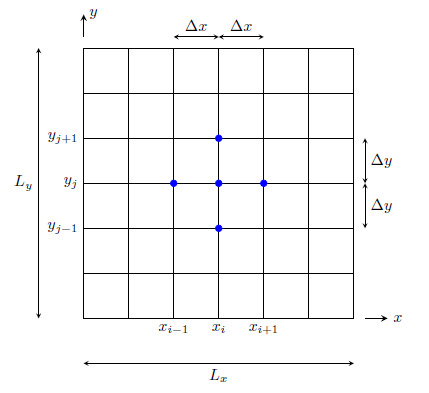
\includegraphics[width=0.8\textwidth]{Figures/finite_difference_picture.jpg}
    \caption{Finite Difference Mesh}
    \label{figure_1}
\end{figure}

After the defining mesh system, certain  $\frac{\partial q}{\partial t}_{i,j}$ parameters are needed. There exists approximate solutions for $\frac{\partial (uq)}{\partial x}_{i,j}$ and $\frac{\partial (vq)}{\partial x}_{i,j}$, which are given by Equations \ref{equation_3} and \ref{equation_4} respectively:

\begin{equation}
\frac{\partial (uq)}{\partial x}_{i,j} \approx
\begin{cases}
    \frac{u(i, j)p(i, j) - u(i-1, j)q(i-1, j)}{x(i, j) - x(i-1, j)}, & \text{for } u(i, j) \geq 0 \\
    \frac{u(i+1, j)p(i+1, j) - u(i, j)q(i, j)}{x(i+1, j) - x(i, j)}, & \text{for } u(i, j) < 0
\end{cases}
\label{equation_3}
\end{equation}

\begin{equation}
\frac{\partial (vq)}{\partial x}_{i,j} \approx
\begin{cases}
    \frac{v(i, j)p(i, j) - v(i-1, j)q(i-1, j)}{y(i, j) - y(i-1, j)}, & \text{for } v(i, j) \geq 0 \\
    \frac{v(i+1, j)p(i+1, j) - v(i, j)q(i, j)}{y(i+1, j) - y(i, j)}, & \text{for } v(i, j) < 0
\end{cases}
\label{equation_4}
\end{equation}





Once $\frac{\partial (vq)}{\partial x}_{i,j}$ and $\frac{\partial (vq)}{\partial x}_{i,j}$ are defined, $\frac{\partial q}{\partial t}_{i,j}$ can be calculated using Equation \ref{equation_5}:             

\begin{equation} % 2D correspondence 
    \frac{\partial q}{\partial t} = \text{rhs}(q) = \left(-\frac{\partial (uq)}{\partial x} + \frac{\partial (vq)}{\partial y}\right) 
    \label{equation_5}
\end{equation}

Subsequently, a low-storage fourth-order five-stage Runge-Kutta(Runge-Kutta 45) method can be employed to integrate the resulting ordinary differential equation \ref{equation_5} in time (Burman and Ern, 2012, \cite{burman2012implicit})
The Runge-Kutta 45 method is a numerical integration technique commonly used for solving ordinary differential equations (ODEs). It is an extension of the classic fourth-order Runge-Kutta (RK4) method. In the RK45 method, the solution to the ODE is advanced through a series of steps using a weighted average of function evaluations at different points within each step. Unlike RK4, which uses a fixed step size, RK45 dynamically adjusts the step size to balance accuracy and computational efficiency.\\

Runge-Kutta 4th Order, 5-Stage formulation is below:

\begin{equation}
\begin{aligned}
    k_1 &= h \cdot f(t_n, y_n), \\
    k_2 &= h \cdot f(t_n + c_2h, y_n + a_{21}k_1), \\
    k_3 &= h \cdot f(t_n + c_3h, y_n + a_{31}k_1 + a_{32}k_2), \\
    k_4 &= h \cdot f(t_n + c_4h, y_n + a_{41}k_1 + a_{42}k_2 + a_{43}k_3), \\
    k_5 &= h \cdot f(t_n + c_5h, y_n + a_{51}k_1 + a_{52}k_2 + a_{53}k_3 + a_{54}k_4), \\
    y_{n+1} &= y_n + b_1k_1 + b_2k_2 + b_3k_3 + b_4k_4 + b_5k_5,
\end{aligned}
\end{equation}

\clearpage
The solver of linear advection code (rhsQ) is given below: 
\definecolor{mygray}{rgb}{0.95,0.95,0.95}
\begin{minted}[autogobble=true, frame=lines, framesep=4mm, baselinestretch=1.2, bgcolor=mygray, fontsize=\footnotesize, linenos=true, breaklines]{c}
void RhsQ(solver_t *solver, tstep_t *tstep, int stage){
mesh_t *msh = &solver->msh;
int n; //variable of n to get rid of (i,j) representation
double dux, dvy, dqt, u, v;
for(int j=0; j<msh->NY; j++){
    for(int i=0; i<msh->NX; i++){
      n=j*msh->NX+i; //calculation of n to get rid of (i,j) representation

      //Calculating u(n) and v(n)
      if (solver->u[n] < 0){
      dux=(solver->q[msh->N2N[4 * n + 1]]*solver->u[msh->N2N[4 * n + 1]]-solver->q[n]*solver->u[n])/(msh->x[1]-msh->x[0]);
      }
      else{
      dux=(solver->q[n]*solver->u[n]-solver->q[msh->N2N[4 * n + 3]]*solver->u[msh->N2N[4 * n + 3]])/(msh->x[1]-msh->x[0]);      
      }
      if (solver->u[n + msh->Nnodes] < 0){
      dvy=(solver->q[msh->N2N[4 * n]]*solver->u[msh->N2N[4 * n]+ msh->Nnodes]-solver->q[n]*solver->u[n+ msh->Nnodes])/(msh->y[msh->NX]-msh->y[0]);
      }
      else{
      dvy=(solver->q[n]*solver->u[n+ msh->Nnodes]-solver->q[msh->N2N[4 * n + 2]]*solver->u[msh->N2N[4 * n + 2]+ msh->Nnodes])/(msh->y[msh->NX]-msh->y[0]);      
      }
      tstep->rhsq[n]=-(dux+dvy); // dq/dt is calculated.

      //Time integration in 2 steps 
      //Step 1: Update residual*/
      //resq = rk4a(stage)* resq + dt*rhsq
      tstep->resq[n] = tstep->rk4a[stage] * tstep->resq[n] + tstep->dt * tstep->rhsq[n];
      //Step:2 Update solution and store
       //q = q + rk4b(stage)*resq
      solver->q[n] = solver->q[n] + tstep->rk4b[stage] * tstep->resq[n];

    }
  }
}
\end{minted}


\clearpage
\subsection{Initial Conditions}
To solve the linear advection equation, initial condition and velocity fields have to be defined at the initial state. The initial values of q, which are transport quantity, are calculated with Equation \ref{equation_6} below:\\
\begin{equation} %2D correspondence 
    \ q = \sqrt{(x - x_{c})^2+(y - y_{c})^2} - r 
    \label{equation_6}
\end{equation}
The velocity of x direction is u and the velocity of y direction is v. They are calculated with Equations~ \ref{equation_7}, \ref{equation_8} below: 

\begin{equation} %2D correspondence 
    \ u = sin(4\pi(x + 0.5))sin(4\pi(y + 0.5)) 
    \label{equation_7}
\end{equation}

\begin{equation} %2D correspondence 
    \ v = cos(4\pi(x + 0.5))cos(4\pi(y + 0.5)) 
    \label{equation_8}
\end{equation}

The initial canditions of linear advection code(initialCondition) is below: 
\definecolor{mygray}{rgb}{0.95,0.95,0.95}
\begin{minted}[autogobble=true, frame=lines, framesep=4mm, baselinestretch=1.2, bgcolor=mygray, fontsize=\footnotesize, linenos=true, breaklines]{c}
void initialCondition(solver_t *solver){
  mesh_t *msh = &(solver->msh); 
  solver->q = (double *)malloc(msh->Nnodes*sizeof(double)); 
  solver->u = (double *)malloc(2*msh->Nnodes*sizeof(double));
  int n;
  double x_c=0.5;
  double y_c=0.75;
  double r=0.15;  
  for(int j=0; j<msh->NY; j++){
    for(int i=0; i<msh->NX; i++){    
     n=j*msh->NX+i; //calculation of n to get rid of (i,j) representation
     solver->q[n] = sqrt(pow(msh->x[n] - x_c, 2) + pow(msh->y[n] - y_c, 2)) - r;
     solver->u[n]=sin(4 * M_PI * (msh->x[n] + 0.5)) * sin(4 * M_PI * (msh->y[n] + 0.5) );
     solver->u[n+msh->Nnodes]=cos(4 * M_PI * (msh->x[n] + 0.5) ) * cos(4 * M_PI * (msh->y[n] + 0.5) );
    }
  }
}
\end{minted}

\clearpage
\subsection{Boundaries and Neighbors}

The periodic boundary condition is applied for this equation. At the periodic boundary condition, the node (i; j) is connected to nodes (i+1; j), (i; j +1), (i - 1; j) (i; j - 1) from east, north, west and south directions. The periodic boundary conditions imply that the nodes for (i = 0; j) are connected to (i = NX - 1; j) for j = 0, 1, ...., NY - 1. And similarly, the nodes (j = 0; i) are connected to (j = NY - 1; i) for i = 0, 1, ...., NX - 1. However, for coding, there are 9 different mesh boundary states. The states are shown in Figure \ref{figure_2}. 

\begin{figure}[hbt!]
    \centering
    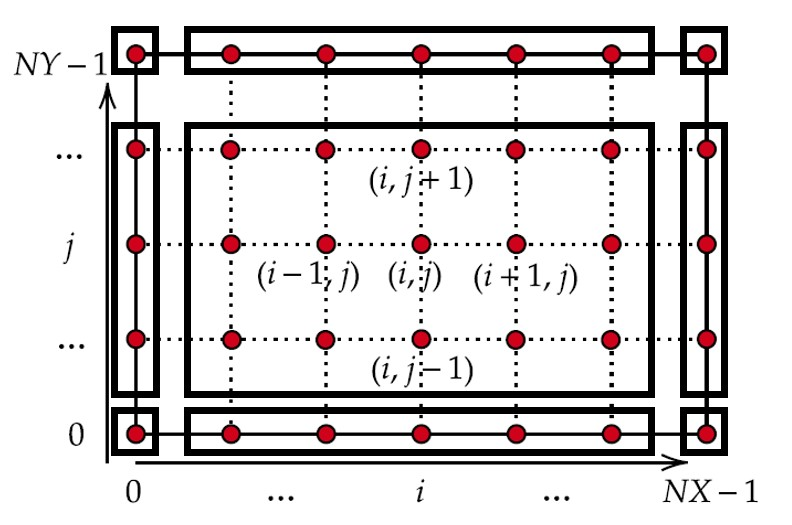
\includegraphics[width=0.8\textwidth]{Figures/boundry_conditions.jpg}
    \caption{Finite Difference Method}
    \label{figure_2}
\end{figure}

So, to define the neighbors and boundaries, the node positions have to be checked. 

For corner nodes, they don't have 2 neighbors. To define these neighbors, the rule explained before is used twice: once for the x-direction and second for the y-direction.

For edges nodes, they don't have 1 neighbor. To define these neighbors, the rule explained before is used once for missing directions.

For inside nodes, they have all neighbors.

To store neighbor positions of each node, linear indices n is used instead of double indices
(i, j). The formulation of linear indices is given in Equation \ref{equation_9}:  
\begin{equation} %2D correspondence 
    \ n = j X NX +i
    \label{equation_9}
\end{equation}

\clearpage
To create mesh and store neighbor positions of each node code(createMesh) is below: 
\definecolor{mygray}{rgb}{0.95,0.95,0.95}
\begin{minted}[autogobble=true, frame=lines, framesep=4mm, baselinestretch=1.2, bgcolor=mygray, fontsize=\footnotesize, linenos=true, breaklines]{c}
mesh_t createMesh(char* inputFile){
  mesh_t msh; 
  // Read required fields i.e. NX, NY, XMIN, XMAX, YMIN, YMAX
  msh.NX   = readInputFile(inputFile, "NX");
  msh.NY   = readInputFile(inputFile, "NY");
  msh.xmin   = readInputFile(inputFile, "XMIN");
  msh.xmax   = readInputFile(inputFile, "XMAX");
  msh.ymin   = readInputFile(inputFile, "YMIN");
  msh.ymax   = readInputFile(inputFile, "YMAX");
  msh.Nnodes = msh.NX*msh.NY;
  msh.x = (double *) malloc(msh.Nnodes*sizeof(double));
  msh.y = (double *) malloc(msh.Nnodes*sizeof(double));
  //Compute Coordinates of the nodes
  double x_interval=(msh.xmax-msh.xmin)/(msh.NX-1); //horizontal interval between two nodes 
  double y_interval=(msh.ymax-msh.ymin)/(msh.NY-1); //vertical interval between two nodes 
  //double grid_array[msh.NX*msh.NY][2]; //creating array for calculating positions of nodes , x-->row , y--> column 
  int n;
  for(int j=0; j<msh.NY; j++){
    for(int i=0; i<msh.NX; i++){
    n=j*msh.NX+i; //calculation of n to get rid of (i,j) representation
    msh.x[n]=i*x_interval; //x coordinates of nodes
    msh.y[n]=j*y_interval; //y coordinates of nodes 
    } }
 //For every node 4 connections East north west and South-North that periodic connections required specific treatment
  msh.N2N = (int *)malloc(4*msh.Nnodes*sizeof(int)); // yukarı-->0, sağ-->1, aşağı-->2, sol-->3 
  for(int j=0; j<msh.NY; j++){
    for(int i=0; i<msh.NX; i++){
    n=j*msh.NX+i;
      if(i==0 && j!=0 && j!=msh.NY-1){
        //left side
        msh.N2N[4*n]=n+msh.NX; 
        msh.N2N[4*n+1]=n+1;
        msh.N2N[4*n+2]=n-msh.NX; 
        msh.N2N[4*n+3]=n+msh.NX-1; 
      }else if (j==0 && i!=0 && i!=msh.NX-1){
        //bottom side
        msh.N2N[4*n]=n+msh.NX; 
        msh.N2N[4*n+1]=n+1;
        msh.N2N[4*n+2]=((msh.NY-1)*msh.NX)+i; 
        msh.N2N[4*n+3]=n-1; 
      }else if (i==msh.NX-1 && j!=0 && j!=msh.NY-1){
        //right side 
        msh.N2N[4*n]=n+msh.NX; 
        msh.N2N[4*n+1]=(n-msh.NX)+1;
        msh.N2N[4*n+2]=n-msh.NX; 
        msh.N2N[4*n+3]=n-1; 
      }else if (j==msh.NY-1 && i!=0 && i!=msh.NX-1){
        //upper side 
        msh.N2N[4*n]=i; 
        msh.N2N[4*n+1]=n+1;
        msh.N2N[4*n+2]=n-msh.NX; 
        msh.N2N[4*n+3]=n-1; 
      }else if(i==0&&j==0){
        //bottom left corner 
        msh.N2N[4*n]=n+msh.NX; 
        msh.N2N[4*n+1]=n+1;
        msh.N2N[4*n+2]=((msh.NY-1)*msh.NX); 
        msh.N2N[4*n+3]=(n+(msh.NX))-1; 
      }else if (i==msh.NX-1 && j==0){
        //bottom right corner 
        msh.N2N[4*n]=n+msh.NX; 
        msh.N2N[4*n+1]=(n-msh.NX)+1;
        msh.N2N[4*n+2]=((msh.NY-1)*msh.NX)+(msh.NX-1); 
        msh.N2N[4*n+3]=n-1; 
      }else if (j==msh.NY-1 && i==0){
        //top left corner 
        msh.N2N[4*n]=0; 
        msh.N2N[4*n+1]=n+1;
        msh.N2N[4*n+2]=n-msh.NX; 
        msh.N2N[4*n+3]=(msh.NX*msh.NY)-1;
      }else if (j==msh.NY-1 && i==msh.NX-1){
        //top right corner 
        msh.N2N[4*n]=i; 
        msh.N2N[4*n+1]=(n-msh.NX)+1;
        msh.N2N[4*n+2]=n-msh.NX; 
        msh.N2N[4*n+3]=n-1;
      } else {
        //inner
        msh.N2N[4*n]=n+msh.NX; 
        msh.N2N[4*n+1]=n+1;
        msh.N2N[4*n+2]=n-(msh.NX); 
        msh.N2N[4*n+3]=n-1;
      } } }
return msh; 
}
\end{minted}


\clearpage
\section{Results}
The analysis is conducted with 3 different time steps and 6 different mesh sizes. These analyses are presented in Table \ref{tab:label1} below: 
\begin{table}[htbp] % Required for table
\caption{List of Analysis}
  \centering
  \begin{tabular}{|c|c|}
    \hline
     Time step& Mesh resolution  \\
    \hline
    \multirow{6}{*}{1e-4} & 20*20 \\
                         & 40*40 \\
                         & 80*80 \\
                         & 160*160 \\
                         & 320*320 \\
                         & 400*400 \\
    \hline
    \multirow{6}{*}{5e-5} & 20*20 \\
                         & 40*40 \\
                         & 80*80 \\
                         & 160*160 \\
                         & 320*320 \\
                         & 400*400 \\
    \hline
    \multirow{6}{*}{1e-5} & 20*20 \\
                         & 40*40 \\
                         & 80*80 \\
                         & 160*160 \\
                         & 320*320 \\
                         & 400*400 \\
    \hline
  \end{tabular}
  \label{tab:label1}  
\end{table}

The procedure for selecting the time step and mesh resolution involves initially employing a larger time step and lower mesh resolution. Subsequently, the mesh resolution is incrementally increased while maintaining the same time step. Once all desired mesh resolutions have been evaluated, the time step is reduced, and the entire analysis is repeated. \\

The results are below for each time step and mesh resolution from Figure \ref{t1m1_1} to Figure \ref{t3m6_2}.


\clearpage
\subsection{Time step:1e-4}

The chosen mesh resolutions are below: 

\subsubsection{Mesh 20*20}

\begin{figure}[hbt!]
  \begin{subfigure}{0.5\textwidth}
        \centering
        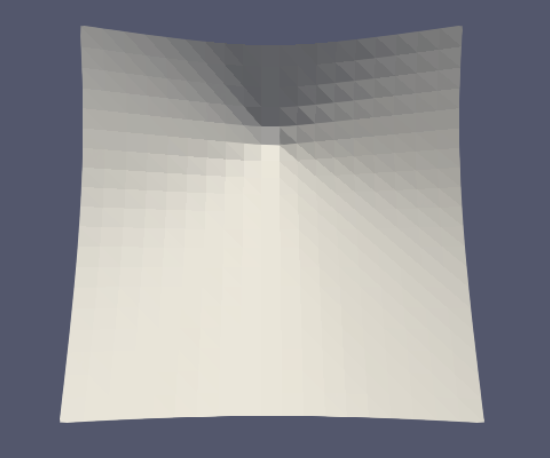
\includegraphics[width=\textwidth]{Figures/e-4 20x20/for n 1.png}
        \caption{Initial field}
  \end{subfigure}
  \hfill
  \begin{subfigure}{0.4\textwidth}
        \centering
        
\includegraphics[width=\textwidth]{Figures/e-4 20x20/for n 10.png}
        \caption{Final field}
  \end{subfigure}
  \caption{Time step is 1e-4}
  \label{t1m1_1} 
\end{figure}

\begin{figure}[hbt!]
    \centering
    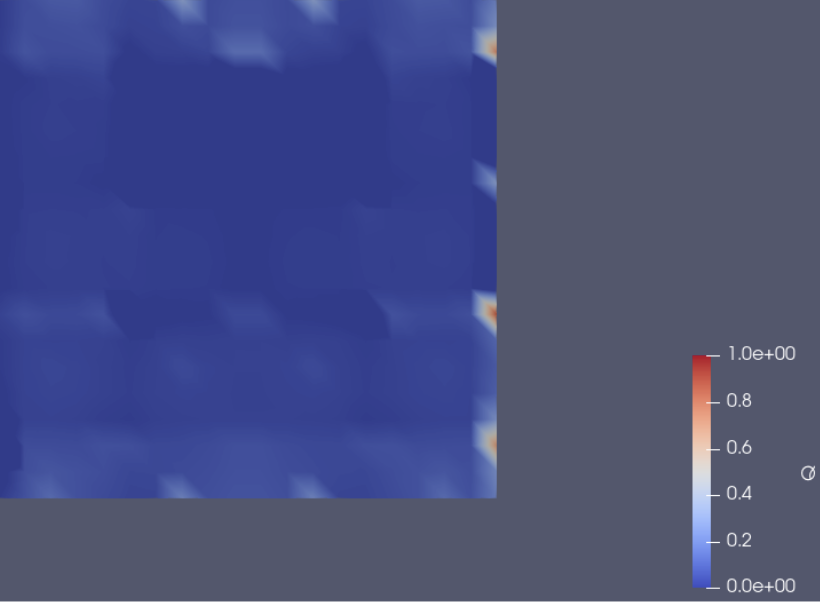
\includegraphics[width=0.5\textwidth]{Figures/e-4 20x20/contour.png}
    \caption{The contour final field for time step 1e-4}
    \label{t1m1_2} 
\end{figure}

As seen from Figure \ref{t1m1_1} to Figure \ref{t1m1_2}, resolution is not enough. 


\clearpage
\subsubsection{Mesh 40*40}
\begin{figure}[hbt!]
  \begin{subfigure}{0.4\textwidth}
        \centering
        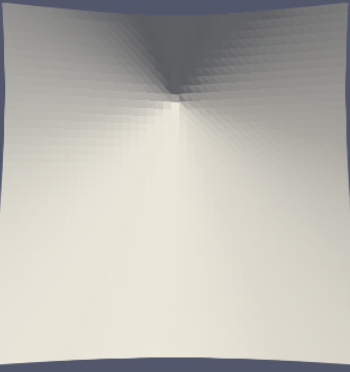
\includegraphics[width=\textwidth]{Figures/e-4 40x40/for n 1.png}
        \caption{Initial field}
  \end{subfigure}
  \hfill
  \begin{subfigure}{0.4\textwidth}
        \centering
        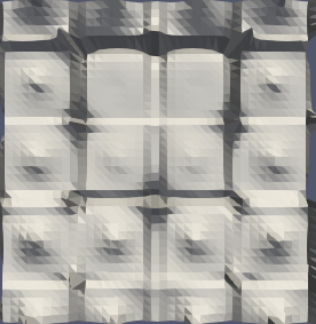
\includegraphics[width=\textwidth]{Figures/e-4 40x40/for n 10.png}
        \caption{Final field}
  \end{subfigure}
  \caption{Time step is 1e-4}
  \label{t1m2_1} 
\end{figure}

\begin{figure}[hbt!]
    \centering
    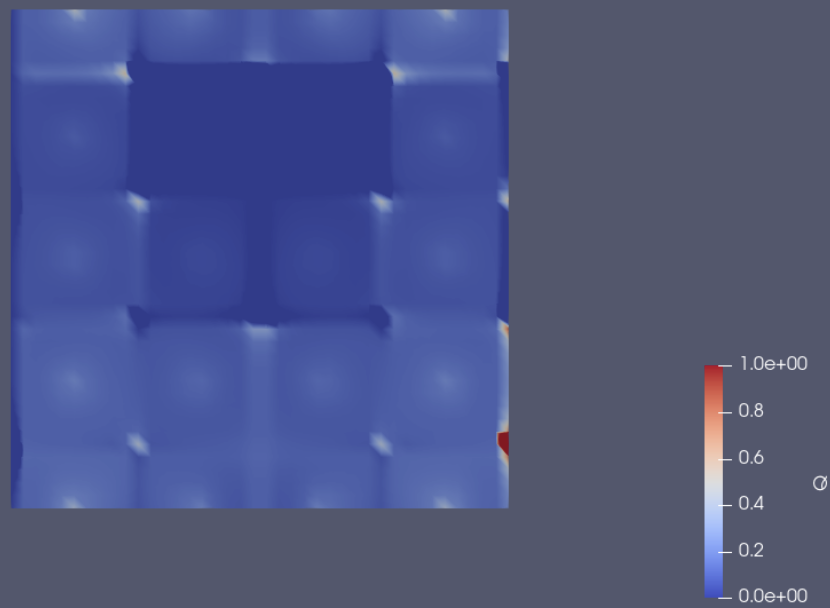
\includegraphics[width=0.5\textwidth]{Figures/e-4 40x40/contour.png}
    \caption{The contour final field for time step 1e-4}
    \label{t1m2_2} 
\end{figure}

As seen from Figure \ref{t1m2_1} to Figure \ref{t1m2_2}, resolution is not enough. 

\clearpage
\subsubsection{Mesh 80*80}
\begin{figure}[hbt!]
  \begin{subfigure}{0.4\textwidth}
        \centering
        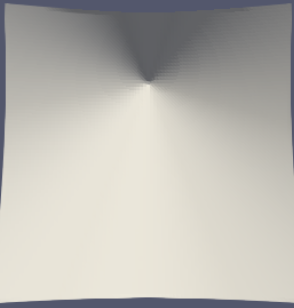
\includegraphics[width=\textwidth]{Figures/e-4 80x80/for n 1.png}
        \caption{Initial field}
  \end{subfigure}
  \hfill
  \begin{subfigure}{0.4\textwidth}
        \centering
        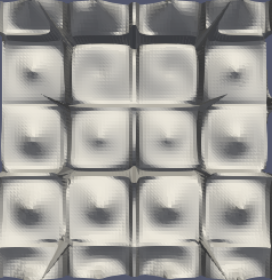
\includegraphics[width=\textwidth]{Figures/e-4 80x80/for n 10.png}
        \caption{Final field}
  \end{subfigure}
  \caption{Time step is 1e-4}
  \label{t1m3_1} 
\end{figure}

\begin{figure}[hbt!]
    \centering
    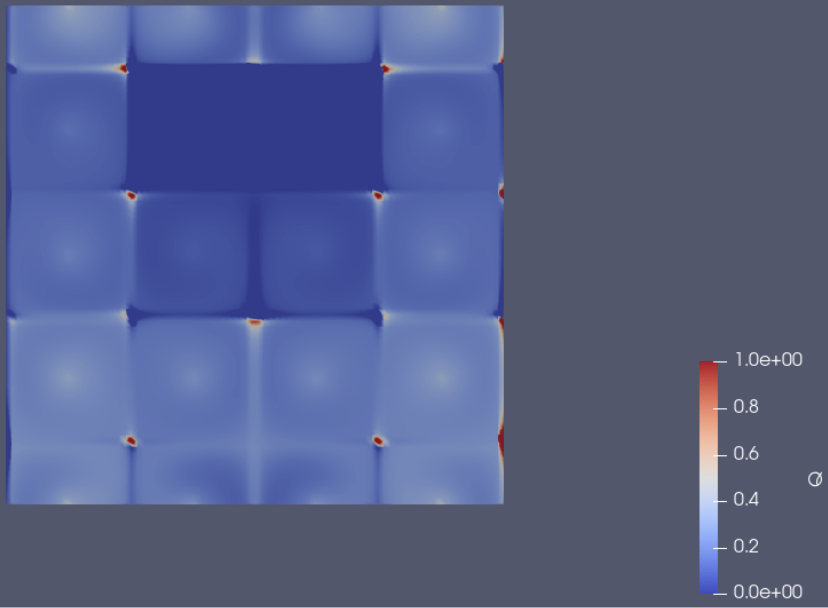
\includegraphics[width=0.5\textwidth]{Figures/e-4 80x80/contour.png}
    \caption{The contour final field for time step 1e-4}
    \label{t1m3_2} 
\end{figure}

As seen from Figure \ref{t1m3_1} to Figure \ref{t1m3_2}, resolution is better but still not enough.


\clearpage
\subsubsection{Mesh 160*160}
\begin{figure}[hbt!]
  \begin{subfigure}{0.4\textwidth}
        \centering
        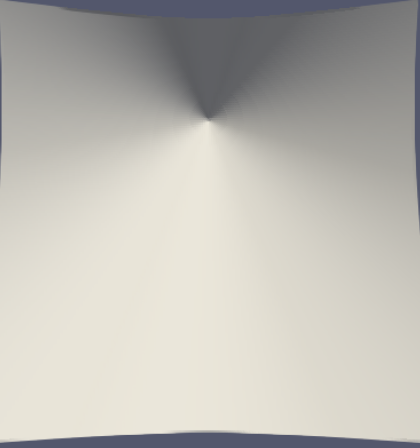
\includegraphics[width=\textwidth]{Figures/e-4 160x160/for n 1.png}
        \caption{Initial field}
  \end{subfigure}
  \hfill
  \begin{subfigure}{0.4\textwidth}
        \centering
        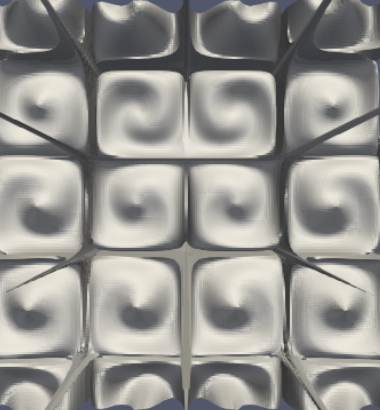
\includegraphics[width=\textwidth]{Figures/e-4 160x160/for n 10.png}
        \caption{Final field}
  \end{subfigure}
  \caption{Time step is 1e-4}
  \label{t1m4_1} 
\end{figure}

\begin{figure}[hbt!]
    \centering
    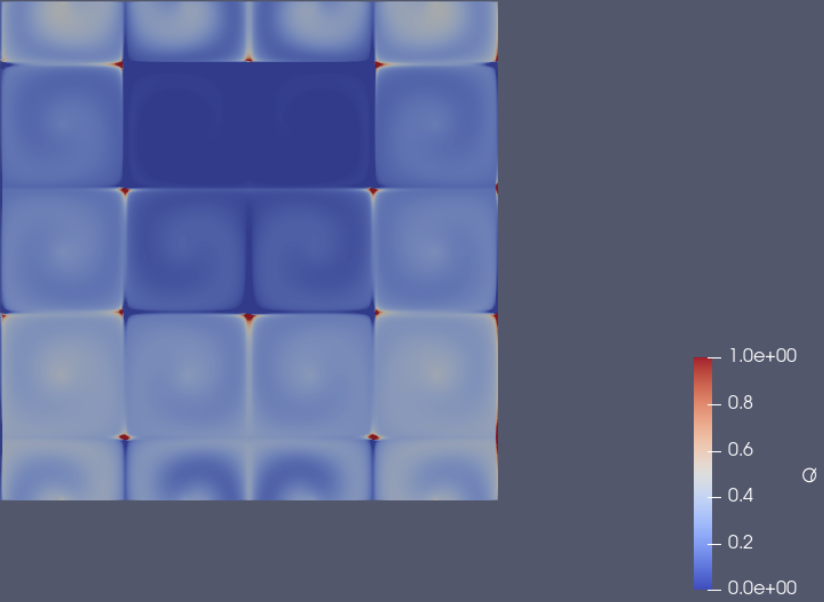
\includegraphics[width=0.5\textwidth]{Figures/e-4 160x160/contour.png}
    \caption{The contour final field for time step 1e-4}
    \label{t1m4_2} 
\end{figure}

As seen from Figure \ref{t1m4_1} to Figure \ref{t1m4_2}, resolution is better.



\clearpage
\subsubsection{Mesh 320*320}
\begin{figure}[hbt!]
  \begin{subfigure}{0.4\textwidth}
        \centering
        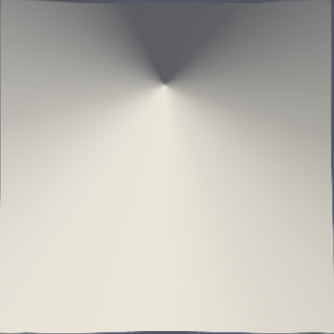
\includegraphics[width=\textwidth]{Figures/e-4 320x320/for n1 .png}
        \caption{Initial field}
  \end{subfigure}
  \hfill
  \begin{subfigure}{0.4\textwidth}
        \centering
        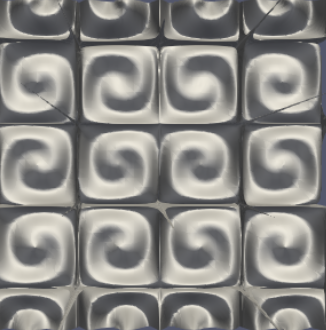
\includegraphics[width=\textwidth]{Figures/e-4 320x320/for n 10.png}
        \caption{Final field}
  \end{subfigure}
  \caption{Time step is 1e-4}
  \label{t1m5_1} 
\end{figure}

\begin{figure}[hbt!]
    \centering
    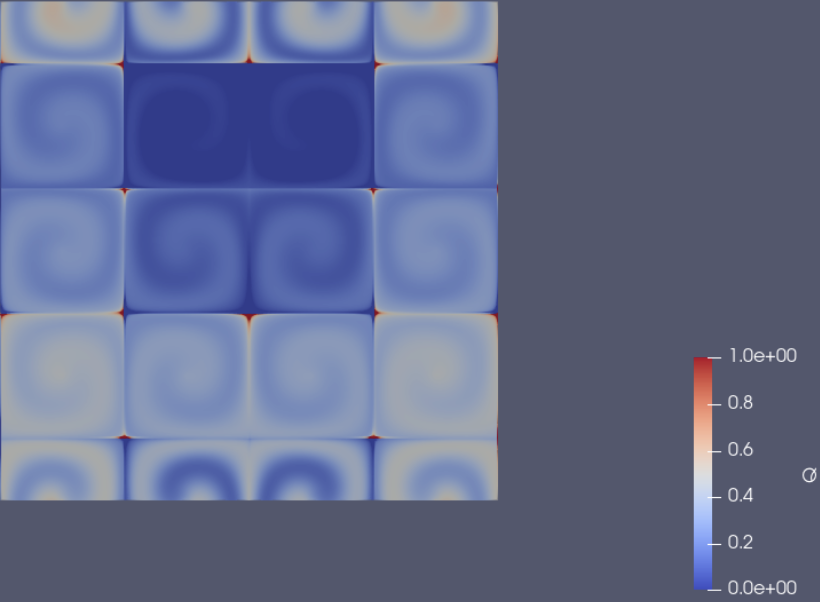
\includegraphics[width=0.5\textwidth]{Figures/e-4 320x320/contour.png}
    \caption{The contour final field for time step 1e-4}
    \label{t1m5_2} 
\end{figure}

As seen from Figure \ref{t1m5_1} to Figure \ref{t1m5_2}, resolution is good.



\clearpage
\subsubsection{Mesh 400*400}
\begin{figure}[hbt!]
  \begin{subfigure}{0.4\textwidth}
        \centering
        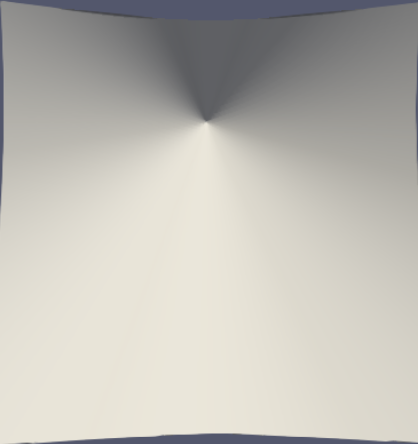
\includegraphics[width=\textwidth]{Figures/e-4 400x400/for n 1.png}
        \caption{Initial field}
  \end{subfigure}
  \hfill
  \begin{subfigure}{0.4\textwidth}
        \centering
        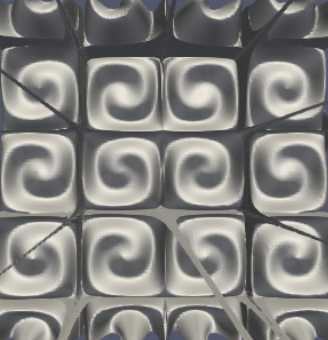
\includegraphics[width=\textwidth]{Figures/e-4 400x400/for n 10.png}
        \caption{Final field}
  \end{subfigure}
  \caption{Time step is 1e-4}
  \label{t1m6_1} 
\end{figure}

\begin{figure}[hbt!]
    \centering
    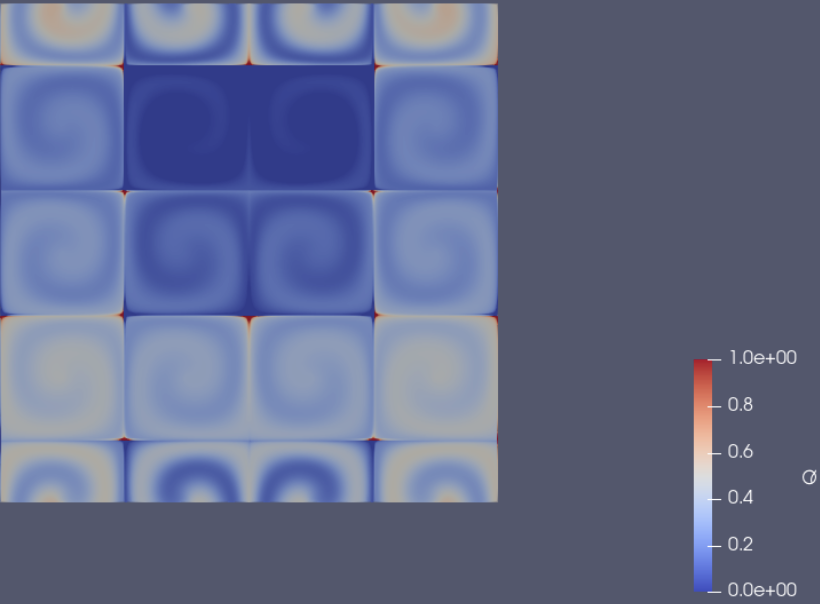
\includegraphics[width=0.5\textwidth]{Figures/e-4 400x400/contour.png}
    \caption{The contour final field for time step 1e-4}
    \label{t1m6_2} 
\end{figure}

As seen from Figure \ref{t1m6_1} to Figure \ref{t1m6_2}, resolution is good and adequate.


\clearpage
\subsection{Time step:5e-5}

The chosen mesh resolutions are below: 

\subsubsection{Mesh 20*20}

\begin{figure}[hbt!]
  \begin{subfigure}{0.5\textwidth}
        \centering
        
\includegraphics[width=\textwidth]{Figures/5e-5 20x20/for n 1.png}
        \caption{Initial field}
  \end{subfigure}
  \hfill
  \begin{subfigure}{0.4\textwidth}
        \centering
        
\includegraphics[width=\textwidth]{Figures/5e-5 20x20/for n 20.png}
        \caption{Final field}
  \end{subfigure}
  \caption{Time step is 5e-5}
  \label{t2m1_1} 
\end{figure}

\begin{figure}[hbt!]
    \centering
    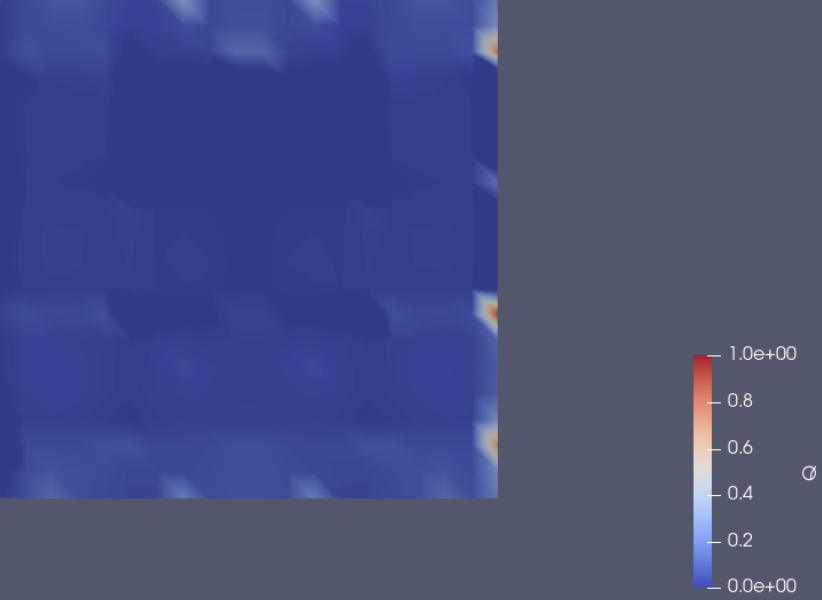
\includegraphics[width=0.5\textwidth]{Figures/5e-5 20x20/contour.png}
    \caption{The contour final field for time step 5e-5}
    \label{t2m1_2} 
\end{figure}

As seen from Figure \ref{t2m1_1} to Figure \ref{t2m1_2}, resolution is not enough. 


\clearpage
\subsubsection{Mesh 40*40}
\begin{figure}[hbt!]
  \begin{subfigure}{0.4\textwidth}
        \centering
        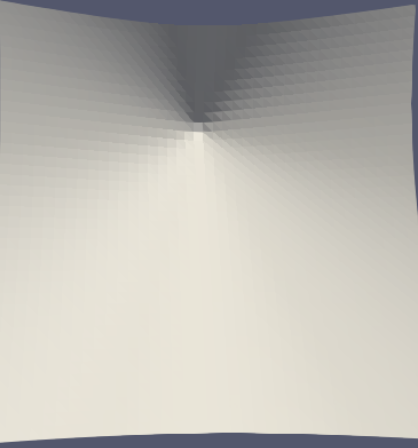
\includegraphics[width=\textwidth]{Figures/5e-5 40x40/for n 1.png}
        \caption{Initial field}
  \end{subfigure}
  \hfill
  \begin{subfigure}{0.4\textwidth}
        \centering
        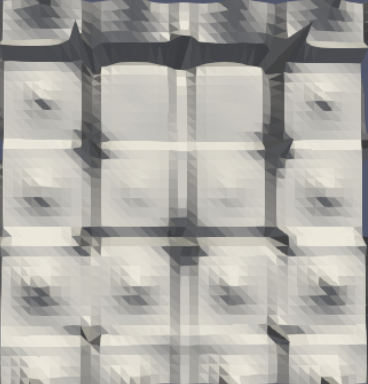
\includegraphics[width=\textwidth]{Figures/5e-5 40x40/for n 20.png}
        \caption{Final field}
  \end{subfigure}
  \caption{Time step is 5e-5}
  \label{t2m2_1} 
\end{figure}

\begin{figure}[hbt!]
    \centering
    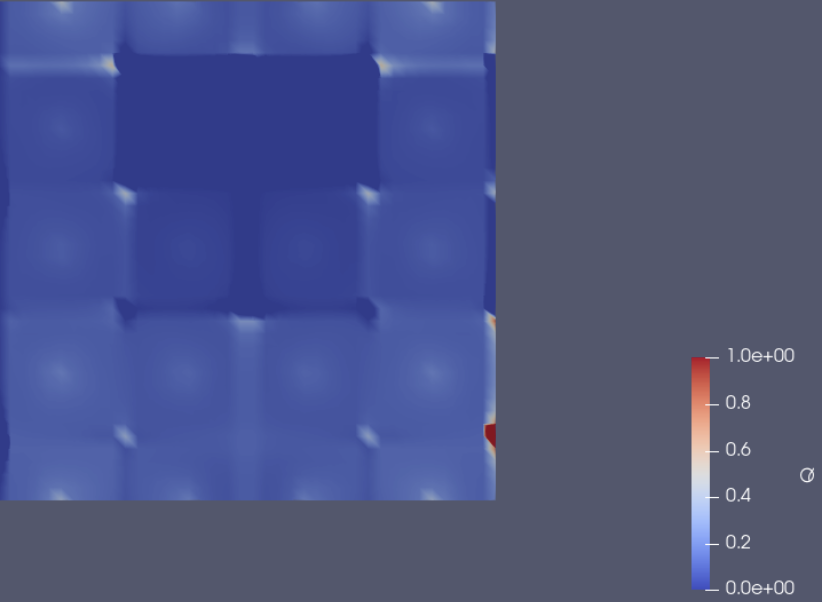
\includegraphics[width=0.5\textwidth]{Figures/5e-5 40x40/contour.png}
    \caption{The contour final field for time step 1e-4}
    \label{t2m2_2} 
\end{figure}

As seen from Figure \ref{t2m2_1} to Figure \ref{t2m2_2}, resolution is not enough. 

\clearpage
\subsubsection{Mesh 80*80}
\begin{figure}[hbt!]
  \begin{subfigure}{0.4\textwidth}
        \centering
        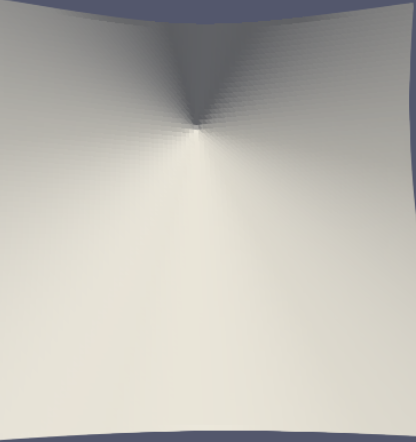
\includegraphics[width=\textwidth]{Figures/5e-5 80x80/for n 1.png}
        \caption{Initial field}
  \end{subfigure}
  \hfill
  \begin{subfigure}{0.4\textwidth}
        \centering
        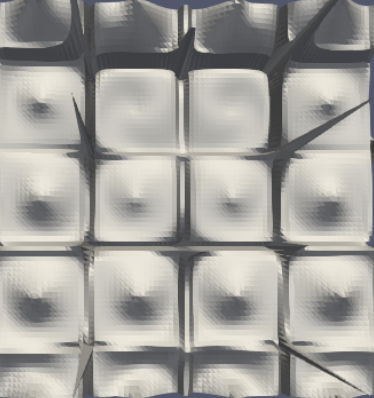
\includegraphics[width=\textwidth]{Figures/5e-5 80x80/for n 20.png}
        \caption{Final field}
  \end{subfigure}
  \caption{Time step is 5e-5}
  \label{t2m3_1} 
\end{figure}

\begin{figure}[hbt!]
    \centering
    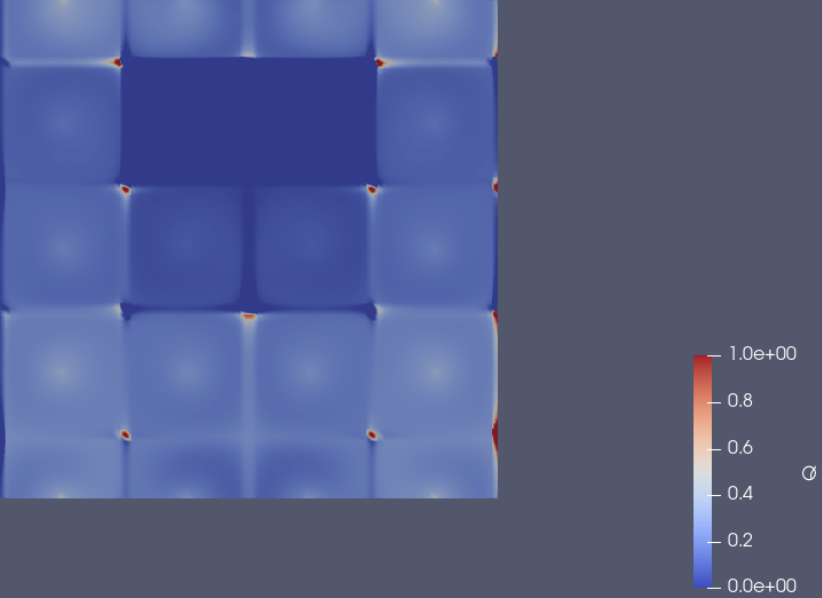
\includegraphics[width=0.5\textwidth]{Figures/5e-5 80x80/contour.png}
    \caption{The contour final field for time step 5e-5}
    \label{t2m3_2} 
\end{figure}

As seen from Figure \ref{t2m3_1} to Figure \ref{t2m3_2}, resolution is not enough.


\clearpage
\subsubsection{Mesh 160*160}
\begin{figure}[hbt!]
  \begin{subfigure}{0.4\textwidth}
        \centering
        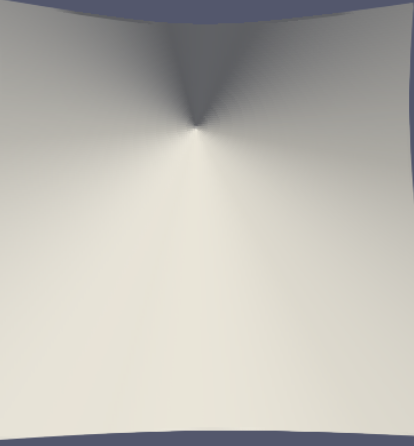
\includegraphics[width=\textwidth]{Figures/5e-5 160x160/for n 1.png}
        \caption{Initial field}
  \end{subfigure}
  \hfill
  \begin{subfigure}{0.4\textwidth}
        \centering
        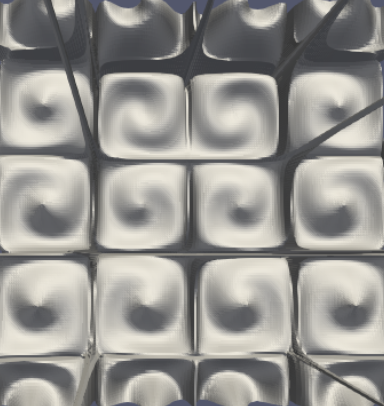
\includegraphics[width=\textwidth]{Figures/5e-5 160x160/for n 20.png}
        \caption{Final field}
  \end{subfigure}
  \caption{Time step is 5e-5}
  \label{t2m4_1} 
\end{figure}

\begin{figure}[hbt!]
    \centering
    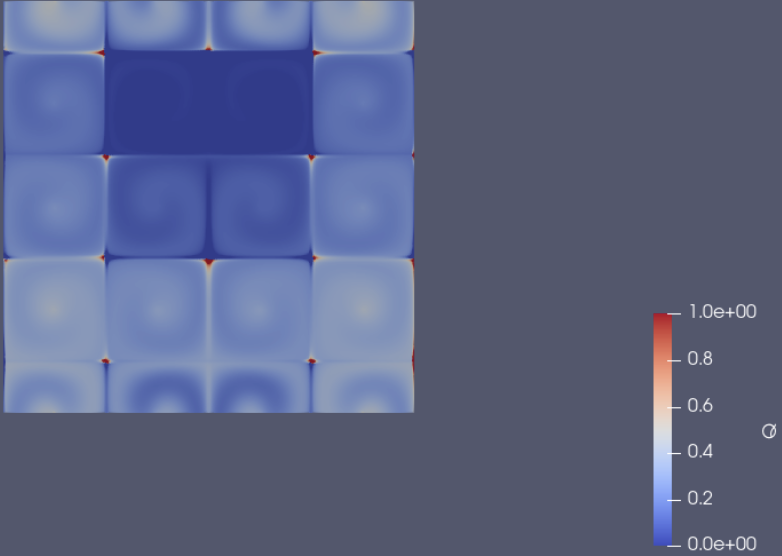
\includegraphics[width=0.5\textwidth]{Figures/5e-5 160x160/contour.png}
    \caption{The contour final field for time step 5e-5}
    \label{t2m4_2} 
\end{figure}

As seen from Figure \ref{t2m4_1} to Figure \ref{t2m4_2}, resolution is better but there are still regions in which it is not adequate.



\clearpage
\subsubsection{Mesh 320*320}
\begin{figure}[hbt!]
  \begin{subfigure}{0.4\textwidth}
        \centering
        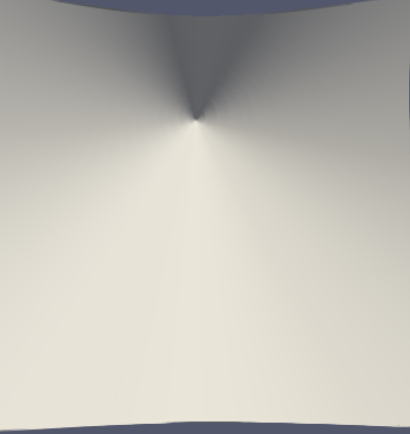
\includegraphics[width=\textwidth]{Figures/5e-5 320x320/for n 1.png}
        \caption{Initial field}
  \end{subfigure}
  \hfill
  \begin{subfigure}{0.4\textwidth}
        \centering
        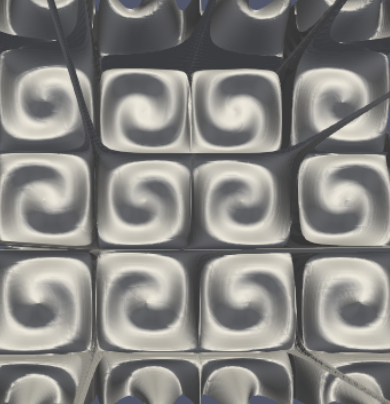
\includegraphics[width=\textwidth]{Figures/5e-5 320x320/for n 20.png}
        \caption{Final field}
  \end{subfigure}
  \caption{Time step is 5e-5}
  \label{t2m5_1} 
\end{figure}

\begin{figure}[hbt!]
    \centering
    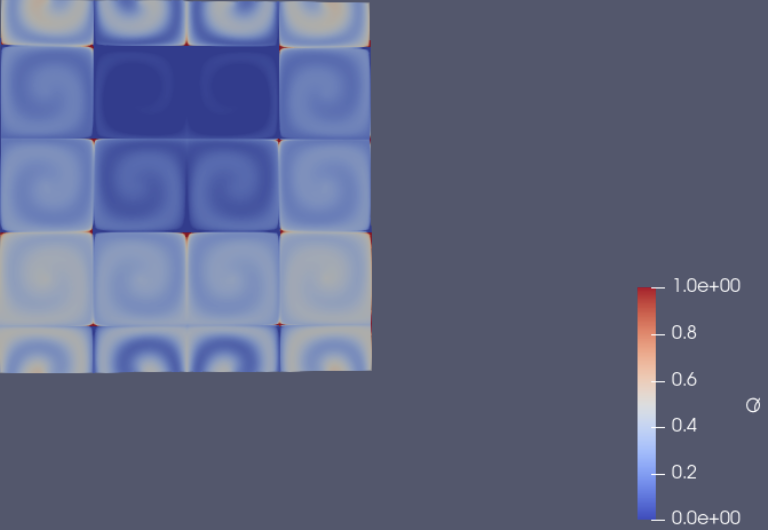
\includegraphics[width=0.5\textwidth]{Figures/5e-5 320x320/contour.png}
    \caption{The contour final field for time step 5e-5}
    \label{t2m5_2} 
\end{figure}

As seen from Figure \ref{t2m5_1} to Figure \ref{t2m5_2}, resolution is good.



\clearpage
\subsubsection{Mesh 400*400}
\begin{figure}[hbt!]
  \begin{subfigure}{0.4\textwidth}
        \centering
        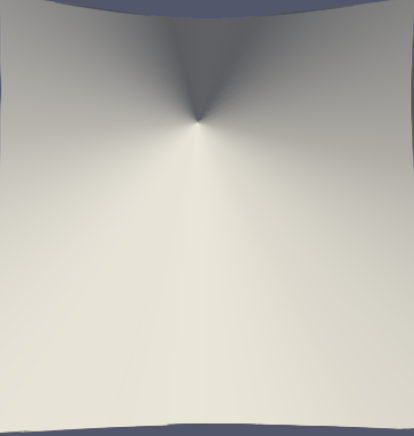
\includegraphics[width=\textwidth]{Figures/5e-5 400x400/for n 1.png}
        \caption{Initial field}
  \end{subfigure}
  \hfill
  \begin{subfigure}{0.4\textwidth}
        \centering
        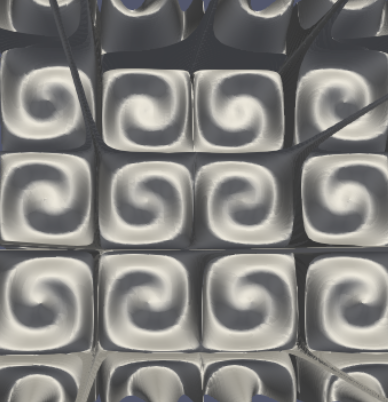
\includegraphics[width=\textwidth]{Figures/5e-5 400x400/for n 20.png}
        \caption{Final field}
  \end{subfigure}
  \caption{Time step is 5e-5}
  \label{t2m6_1} 
\end{figure}

\begin{figure}[hbt!]
    \centering
    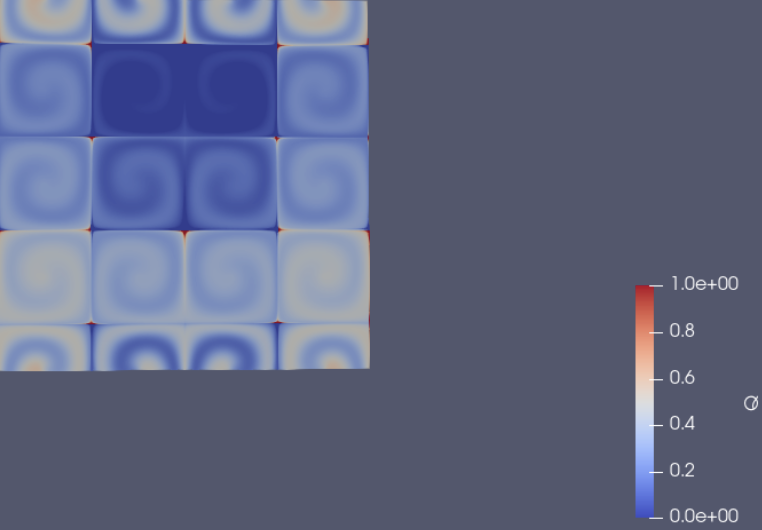
\includegraphics[width=0.5\textwidth]{Figures/5e-5 400x400/contour.png}
    \caption{The contour final field for time step 5e-5}
    \label{t2m6_2} 
\end{figure}

As seen from Figure \ref{t2m6_1} to Figure \ref{t2m6_2}, resolution is very good.


\clearpage
\subsection{Time step:1e-5}

The chosen mesh resolutions are below: 

\subsubsection{Mesh 20*20}

\begin{figure}[hbt!]
  \begin{subfigure}{0.5\textwidth}
        \centering
        
\includegraphics[width=\textwidth]{Figures/e-5 20x20/for n 1.png}
        \caption{Initial field}
  \end{subfigure}
  \hfill
  \begin{subfigure}{0.4\textwidth}
        \centering
        
\includegraphics[width=\textwidth]{Figures/e-5 20x20/for n 100.png}
        \caption{Final field}
  \end{subfigure}
  \caption{Time step is 1e-5}
  \label{t3m1_1} 
\end{figure}

\begin{figure}[hbt!]
    \centering
    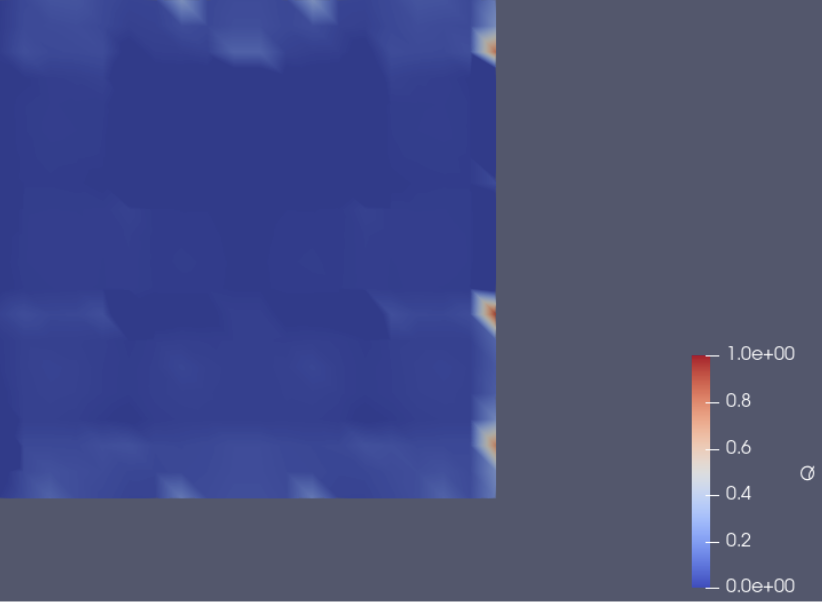
\includegraphics[width=0.5\textwidth]{Figures/e-5 20x20/contour.png}
    \caption{The contour final field for time step 1e-5}
    \label{t3m1_2} 
\end{figure}

As seen from Figure \ref{t3m1_1} to Figure \ref{t3m1_2}, resolution is not enough. 


\clearpage
\subsubsection{Mesh 40*40}
\begin{figure}[hbt!]
  \begin{subfigure}{0.4\textwidth}
        \centering
        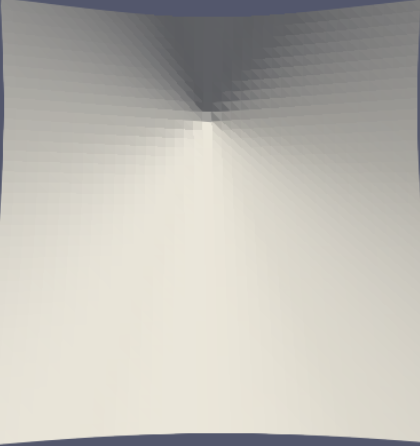
\includegraphics[width=\textwidth]{Figures/e-5 40x40/for n 1.png}
        \caption{Initial field}
  \end{subfigure}
  \hfill
  \begin{subfigure}{0.4\textwidth}
        \centering
        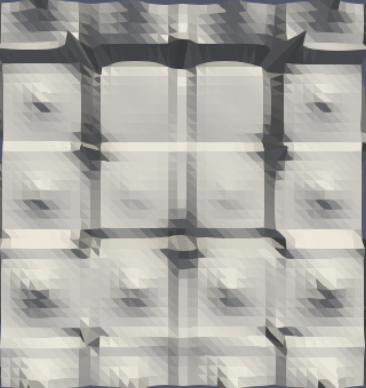
\includegraphics[width=\textwidth]{Figures/e-5 40x40/for n 100.png}
        \caption{Final field}
  \end{subfigure}
  \caption{Time step is 1e-5}
  \label{t3m2_1} 
\end{figure}

\begin{figure}[hbt!]
    \centering
    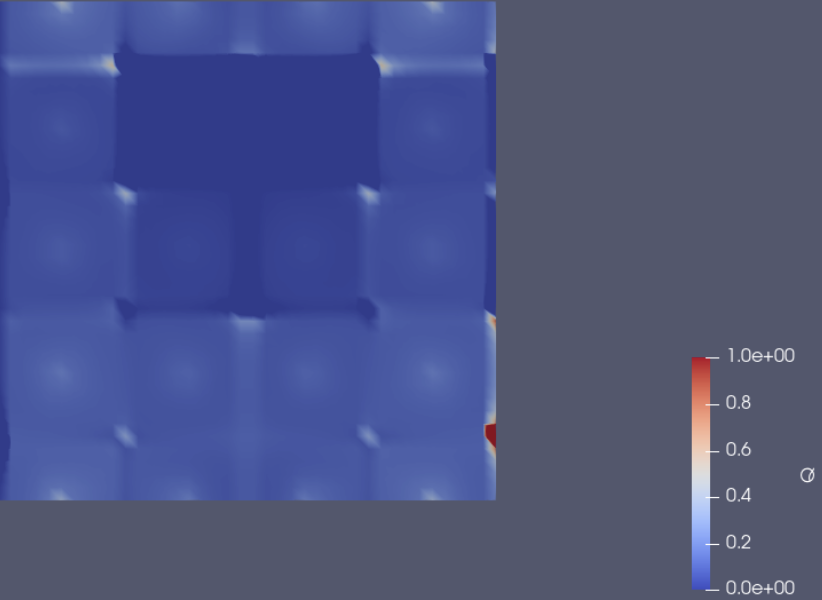
\includegraphics[width=0.5\textwidth]{Figures/e-5 40x40/contour.png}
    \caption{The contour final field for time step 1e-5}
    \label{t3m2_2} 
\end{figure}

As seen from Figure \ref{t3m2_1} to Figure \ref{t3m2_2}, resolution is not enough. 

\clearpage
\subsubsection{Mesh 80*80}
\begin{figure}[hbt!]
  \begin{subfigure}{0.4\textwidth}
        \centering
        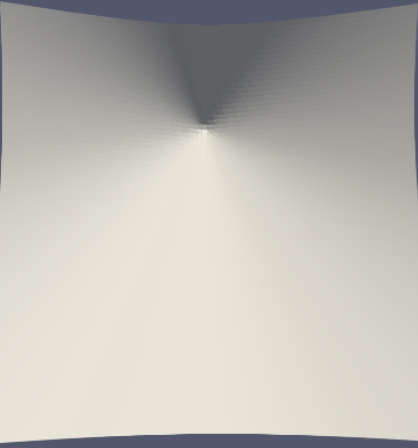
\includegraphics[width=\textwidth]{Figures/e-5 80x80/for n1 .png}
        \caption{Initial field}
  \end{subfigure}
  \hfill
  \begin{subfigure}{0.4\textwidth}
        \centering
        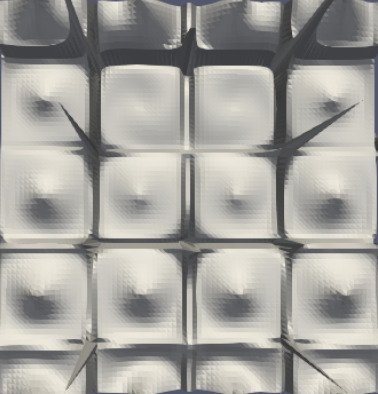
\includegraphics[width=\textwidth]{Figures/e-5 80x80/for n 100.png}
        \caption{Final field}
  \end{subfigure}
  \caption{Time step is 1e-5}
  \label{t3m3_1} 
\end{figure}

\begin{figure}[hbt!]
    \centering
    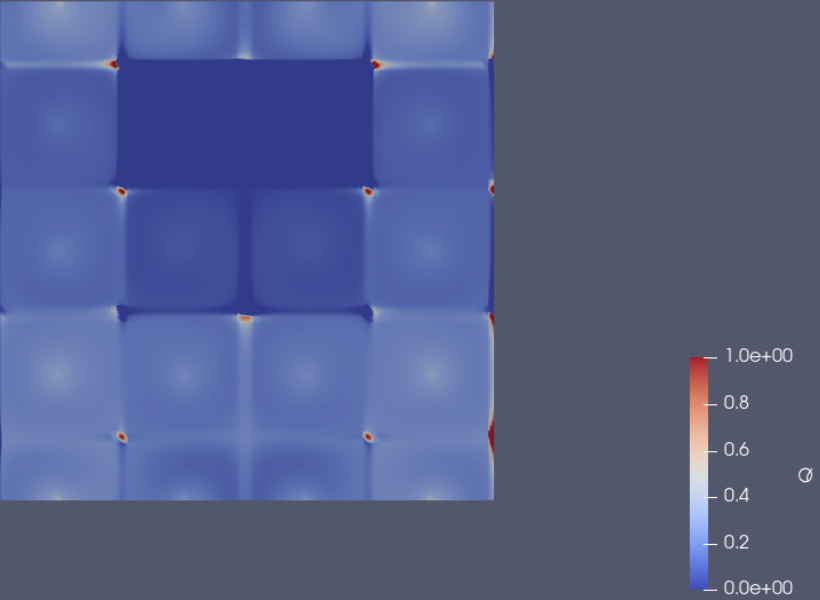
\includegraphics[width=0.5\textwidth]{Figures/e-5 80x80/contour.png}
    \caption{The contour final field for time step 1e-5}
    \label{t3m3_2} 
\end{figure}

As seen from Figure \ref{t3m3_1} to Figure \ref{t3m3_2}, resolution is not enough.


\clearpage
\subsubsection{Mesh 160*160}
\begin{figure}[hbt!]
  \begin{subfigure}{0.4\textwidth}
        \centering
        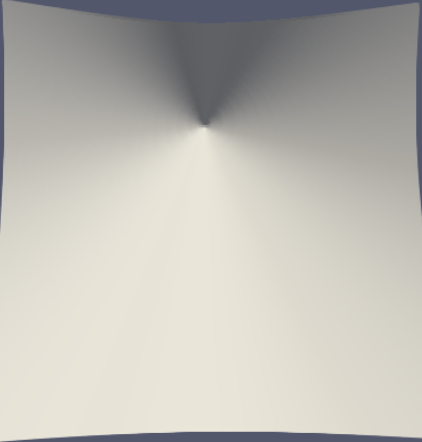
\includegraphics[width=\textwidth]{Figures/e-5 160x160/for n 1.png}
        \caption{Initial field}
  \end{subfigure}
  \hfill
  \begin{subfigure}{0.4\textwidth}
        \centering
        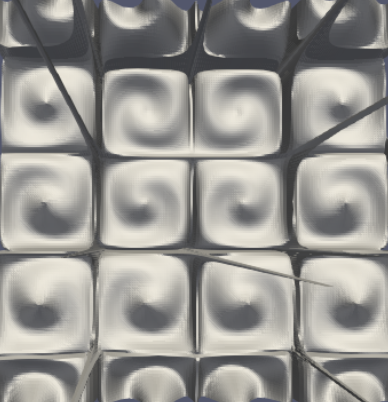
\includegraphics[width=\textwidth]{Figures/e-5 160x160/for n 100.png}
        \caption{Final field}
  \end{subfigure}
  \caption{Time step is 1e-5}
  \label{t3m4_1} 
\end{figure}

\begin{figure}[hbt!]
    \centering
    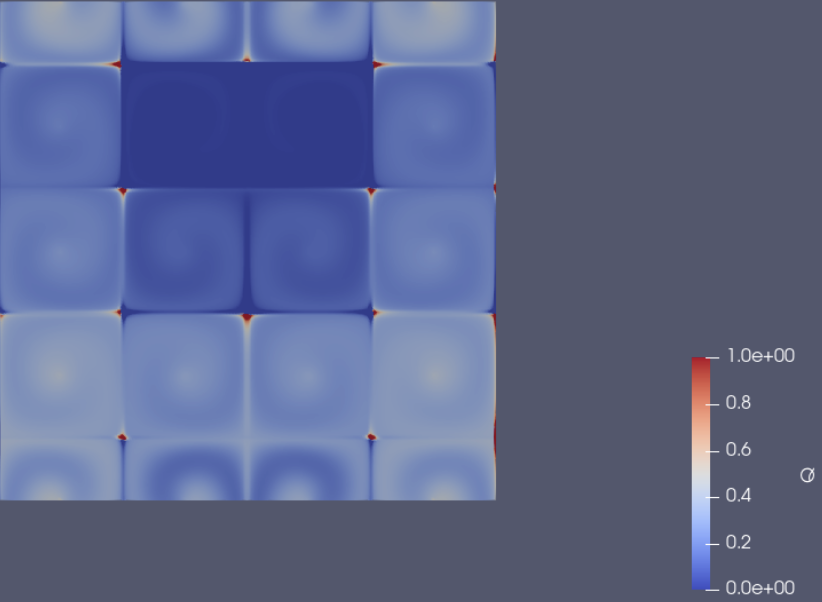
\includegraphics[width=0.5\textwidth]{Figures/e-5 160x160/contour.png}
    \caption{The contour final field for time step 1e-5}
    \label{t3m4_2} 
\end{figure}

As seen from Figure \ref{t3m4_1} to Figure \ref{t3m4_2}, resolution is better.



\clearpage
\subsubsection{Mesh 320*320}
\begin{figure}[hbt!]
  \begin{subfigure}{0.4\textwidth}
        \centering
        \includegraphics[width=\textwidth]{Figures/e-5 320x320/for n 1.png}
        \caption{Initial field}
  \end{subfigure}
  \hfill
  \begin{subfigure}{0.4\textwidth}
        \centering
        \includegraphics[width=\textwidth]{Figures/e-5 320x320/for n 100.png}
        \caption{Final field}
  \end{subfigure}
  \caption{Time step is 1e-5}
  \label{t3m5_1} 
\end{figure}

\begin{figure}[hbt!]
    \centering
    \includegraphics[width=0.5\textwidth]{Figures/e-5 320x320/contour.png}
    \caption{The contour final field for time step 1e-5}
    \label{t3m5_2} 
\end{figure}

As seen from Figure \ref{t3m5_1} to Figure \ref{t3m5_2}, resolution is good.



\clearpage
\subsubsection{Mesh 400*400}
\begin{figure}[hbt!]
  \begin{subfigure}{0.4\textwidth}
        \centering
        \includegraphics[width=\textwidth]{Figures/e-5 400x400/for n 1.png}
        \caption{Initial field}
  \end{subfigure}
  \hfill
  \begin{subfigure}{0.4\textwidth}
        \centering
        \includegraphics[width=\textwidth]{Figures/e-5 400x400/for n 100.png}
        \caption{Final field}
  \end{subfigure}
  \caption{Time step is 1e-5}
  \label{t3m6_1} 
\end{figure}

\begin{figure}[hbt!]
    \centering
    \includegraphics[width=0.5\textwidth]{Figures/e-5 400x400/contour.png}
    \caption{The contour final field for time step 1e-5}
    \label{t3m6_2} 
\end{figure}

As seen from Figure \ref{t3m6_1} to Figure \ref{t3m6_2}, resolution is very good.


\clearpage
\section{Comments and Conclusion}

The biggest effect of the solution is mesh resolution. The results indicate that mesh resolutions, like 20x20, 40x40, and 80x80, are not sufficient for the 2D linear advection solutions across all time steps. This insufficiency is attributed to the characteristics of the velocity fields. We use sinusoidal functions for velocity in both the x and y directions, the sinusoidal function undergoes four cycles, changing from 2π to 6π. To accurately capture this type of function, a higher mesh resolution is necessary, typically around 1 element for every 2-3 degrees. 160*160 and higher resolution solutions support this idea. Although the 160*160 resolution is better, ı prefer 320*320 resolution for acceptable solutions. \\

After choosing the right mesh resolution, results are getting better with decreasing time steps. However, all the time steps are almost the same after choosing the right mesh resolution. This can be seen in Figure \ref{t1m5_2}, \ref{t2m5_2}, \ref{t3m5_2}, 320*320 resolutions are good for all time steps. 


\clearpagepage

\printbibliography
\end{document}


